\subsubsection{ZZ production}
\label{sss-ZZprod}

%short intro
The production of \ZZ in proton-proton collisions has been one of the first di-boson 
processes measured at the LHC. The SM process is an important and irreducible
background to resonance searches and Higgs production. The production at leading
order is dominated by quark anti-quark annihilation in the $t$ and $u$-channel,
whereas the $s$-channel process is forbidden in the SM 
(see Figure~\ref{fig:sss-ZZprod-LOdiagrams}). The gluon fusion process 
contributes about 6\% to the total production cross section. 

%FIGURE LO ZZ DIAGRAM
\begin{figure}[htbp]
  \begin{center}
  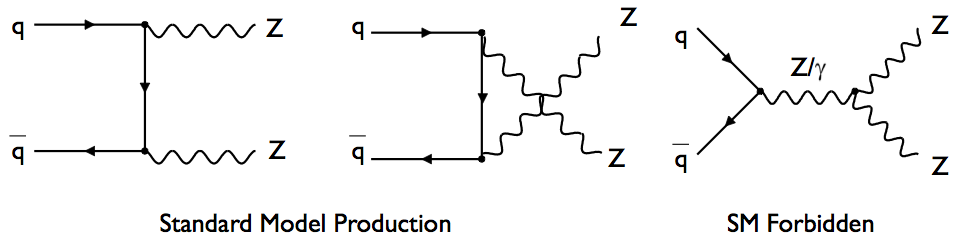
\includegraphics[width=0.6\textwidth]{figures/sss-inclboson-diboson-zzprod-zzdiagram.png}
  \caption{Leading order Feynman diagrams of \ZZ production in the dominant 
  \qqbar\ channel. The production of \ZZ\ via the $s$-channel is forbidden in the SM.}
\label{fig:sss-ZZprod-LOdiagrams}
\end{center}
\end{figure}

%decay channels
Precision measurements use the leptonic decay modes of the $Z$ to reduce the impact of
the QCD background. 
The four lepton final state provides an almost background free signature, at the
expense of a relatively small branching ratio
$\mathcal{B}(ZZ) \to \ll\ll = 0.101^2 \cdot {4 \over 9} = 0.0045$~\cite{Agashe:2014kda}.  
The di-lepton and missing energy channel can exploit the one order-of-magnitude
higher branching ratio of 
$\mathcal{B}(\ZZ \to \ll\vv) = 0.101 \cdot 0.20 \cdot 2 \cdot {2 \over 3} = 0.0269$, 
but has also relatively large backgrounds.

%analysis CMS and ATLAS.
%ATLAS ZZ 7 TeV~\cite{Aad:2012awa}
%CMS ZZ4l 8 TeV~\cite{Khachatryan:2014dia}
%CMS ZZ4l 7 TeV~\cite{Chatrchyan:2012sga}
%CMS ZZ2l2nu 7+8 TeV~\cite{Khachatryan:2015pba}
The ATLAS collaboration has published results on the $7\TeV$ data-set 
in the $\ll\ll$ and $\ll\vv$ final state~\cite{Aad:2012awa}, and at
$13\TeV$ in the $\ll\ll$ final state~\cite{Aad:2015zqe}. The CMS collaboration
has analysed the full 7 and $8\TeV$ data sets in both 
the $\ll\ll$~\cite{Chatrchyan:2012sga,CMS:2014xja} and 
$\ll\vv$ final state~\cite{Khachatryan:2015pba}.
%Theoretical calculations
% NLO alpha_s arXiv:1105.0020
% NLO alpha_EKW arXiv:1305.5402,arXiv:1307.4331
Theoretical predictions for $\ZZ$ production are available 
at NLO in $\alpha_s$~\cite{Campbell:2011bn}. In addition, electroweak 
corrections at NLO have been calculated~\cite{Bierweiler:2013dja,Baglio:2013toa}. 

% Z->llll
%Selections
The event selection for the $\ll\ll$ final state requires exactly four leptons 
fulfilling a set of cuts on kinematic quantities. 
%ATLAS and CMS use similar criteria as listed in detail in Table~\ref{tab:sss-ZZprod-cuts}. 
While ATLAS uses $l=e,\mu$, CMS includes also $\Z\to\tautau$ with subsequent hadronic and leptonic $\tau$
decays. ATLAS uses in addition forward leptons outside the ID tracker
to increase the acceptance by 6\% for electrons and 10\% for muons.
%Backgrounds
The $\ll\ll$ channels offers the cleanest event sample with a background level
of only $2-3\%$ from $\Z+jets$, $\tt$, and di-boson events. 
The background is estimated from data by control regions with looser selection
criteria. 

% Z->llvv
%Selections
Events in the $\ll\vv$ final state are characterized by exactly two leptons 
and missing energy. The event selection requires a $\Z \to \ll$ candidate and
missing energy in the event. Both experiments use refined observables of
missing energy with additional information to improve the rejection 
against instrumental background. 
%Backgrounds 
The background level is of the same order
as the signal and substantially higher than for the $\ll\ll$ channel.
Main background sources are $\V+jets$, $\tt$ and di-boson production. 
ATLAS and CMS use data driven techniques to constrain the 
dominant background sources.

% Results at the end?
% xsec
Besides the total cross section for the $pp \to \ZZ$ production process, both
experiments measure also fiducial and differential cross sections. The results are 
summarized in Tabel~\ref{tab:sss-ZZprod-cross-sections}. ATLAS and CMS
use different definitions of the fiducial phase thus a direct comparison is
not possible.
For the total cross section definition the two experiments differ slightly in the $\Z$ mass range, 
where CMS prefers a wider range of $60\GeV < \mZ < 120\GeV$ than ATLAS with 
$66\GeV < \mZ < 116\GeV$. This difference contributes to the variation in the quoted predicted
cross section. Good agreement between experimental and theoretical cross section
values is observed in both ATLAS and CMS analyses. 


\begin{table}[htp]
\begin{center}
\resizebox{\textwidth}{!}{
\begin{tabular}{|c|c|c|c|c|c|}
 Experiment & decay channel     & \rts & measured $\sigma_{total}$ $[\pb]$                                  & predicted $\sigma_{total}$ $[\pb]$& reference                    \\
 \hline
 ATLAS	     & $\ll\ll$, $\ll\vv$& 7 TeV & {6.7 $\pm$ 0.7 (stat.) $^{+0.4}_{-0.3}$ (syst.) $\pm$ 0.3 (lumi.) }&  6.18$^{+0.25}_{-0.18}$           & \cite{Aad:2012awa}         \\
 CMS	     & $\ll\ll$          & 7 TeV & {6.2 $\pm$ $^{+0.9}_{-0.8}$ (stat.) $^{+0.4}_{-0.3}$ (syst.) $\pm$ 0.1 (lumi.) } & 6.3$\pm 0.4$        & \cite{Chatrchyan:2012sga}  \\
 CMS	     & $\ll\vv$          & 7 TeV & {5.2 $\pm$ $^{+1.5}_{-1.4}$ (stat.) $^{+1.4}_{-1.1}$ (syst.) $\pm$ 0.2 (lumi.) } & 6.1$\pm 0.3$        & \cite{Chatrchyan:2012sga}  \\
 CMS	     & $\ll\ll$          & 8 TeV & {7.7 $\pm$ 0.5 (stat.) $^{+0.5}_{-0.4}$ (syst.) $\pm$ 0.2 (lumi.) } 		        & 7.7$\pm 0.6$        & \cite{CMS:2014xja}         \\ 
 CMS	     & $\ll\vv$          & 8 TeV & {6.9 $\pm$ 0.8 (stat.) $^{+1.8}_{-1.4}$ (syst.) $\pm$ 0.3 (lumi.) }			    & 7.6$\pm 0.3$        & \cite{Chatrchyan:2012sga}  \\% m(ll) > 40GeV, m(vv) > 12GeV
 ATLAS	     & $\ll\ll$			 &13 TeV & {16.7 $\pm$ $^{+2.2}_{-2.0}$ (stat.) $^{+0.9}_{-0.7}$ (syst.) $\pm$ $^{+1.o}_{-0.7}$ (lumi.) }&  15.6$^{+0.4}_{-0.4}$           & \cite{Aad:2015zqe}         \\


\end{tabular}
}
\caption{Summary of measured $\ZZ$ production cross sections from ATLAS and CMS
at 7, 8 and 13 TeV center-of-mass energies in the four lepton and $\ll\vv$ final state.}
\label{tab:sss-ZZprod-cross-sections}
\end{center}
\label{default}
\end{table}%


%%%%
% THIS MIGHT GO INTO THE SECTION ON TGC
% aTGC
% Spectra ATGC
% charged pT : llvv CMS
% m(llll) : llll CMS
% pT(Z) : llll,llvv ATLAS
Limits on ATGC parameters are determined with differential distributions of the 
invariant di-boson mass (CMS, four lepton channel), 
the transverse momentum of the leading lepton (CMS, $\ll\vv$-channel), or
the transverse momentum of the leading \Z (ATLAS, all channels).
For example a comparison of the measured and predicted differential cross sections in bins of the 
four-lepton invariant mass from CMS is shown in Figure \ref{fig:sss-inclboson-diboson-zzprod-zzinvmass}.
The prediction for the case of a non-zero value of the anomalous coupling
parameter $f_4^Z=0.015$ shows an enhancement over the SM value at high 
invariant masses. 

%FIGURE ZZ invariant mass
%1406.0113v2.pdf, FIGURE 5
% https://twiki.cern.ch/twiki/pub/CMSPublic/PhysicsResultsSMP13005/fig5tgcA.pdf
% CMS ZZ 4l 8 TeV
\begin{figure}[htbp]
  \begin{center}
  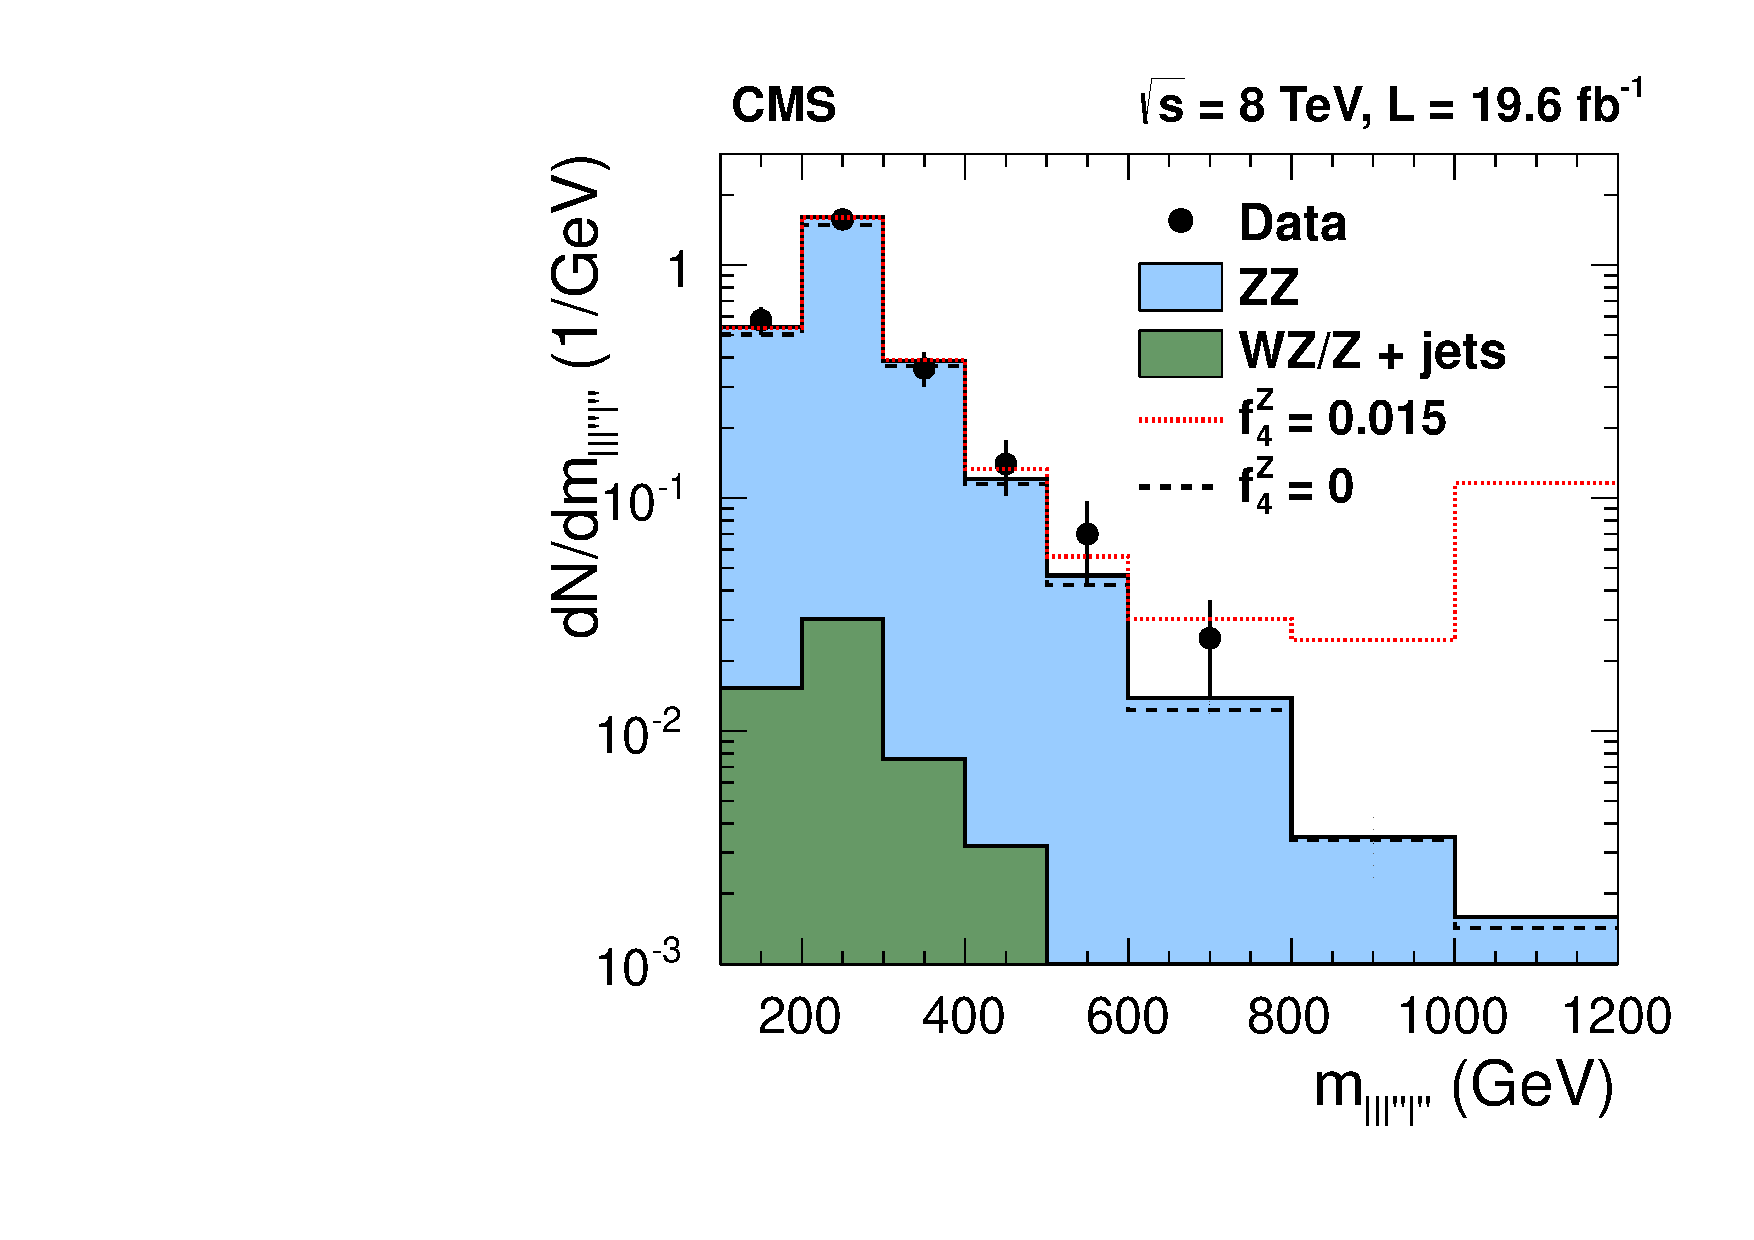
\includegraphics[width=0.4\textwidth]{figures/sss-inclboson-diboson-zzprod-zzinvmass.pdf}
  \caption{ Distribution of the four-lepton reconstructed mass for the combined $4e$, $4\mu$, and $2e2\mu$ channels from CMS~\cite{CMS:2014xja}. Points represent the data, the shaded histogram labeled $\ZZ$ represents the predictions for $\ZZ$ signal, the histograms labeled $\WZ$/$\Z$+jets shows background estimated form data. The dashed and dotted histograms indicate the SM expectation (f4Z = 0) and in the presence of an ATGC (f4Z = 0.015) with all the other anomalous couplings set to zero. The last bin includes all entries with masses above 1000 GeV.
}
\label{fig:sss-inclboson-diboson-zzprod-zzinvmass}
\end{center}
\end{figure}

Both experiments publish 95\% CL limits on ATGC without form factors in the $\ll\ll$ 
and $\ll\vv$ channels. The results are in agreement with the SM and 
summarized in Figure~\ref{fig:sss-inclboson-diboson-zzprod-aTGC_naTGCf} 
taken from Ref. \cite{aTGCplots}. The precision of the LHC results is driven by the steep increase of 
sensitivity with higher center-of-mass energy
and are about 2 orders-of-magnitude better compared to the 
combined LEP result~\cite{LEP-comb-2002}.  
% FIGURE COMPARISON OF ZZ NTGC
% https://twiki.cern.ch/twiki/bin/view/CMSPublic/PhysicsResultsSMPaTGC
% M Herndon
% FETCHED 34RD JULY 2015
\begin{figure}[htbp]
  \begin{center}
  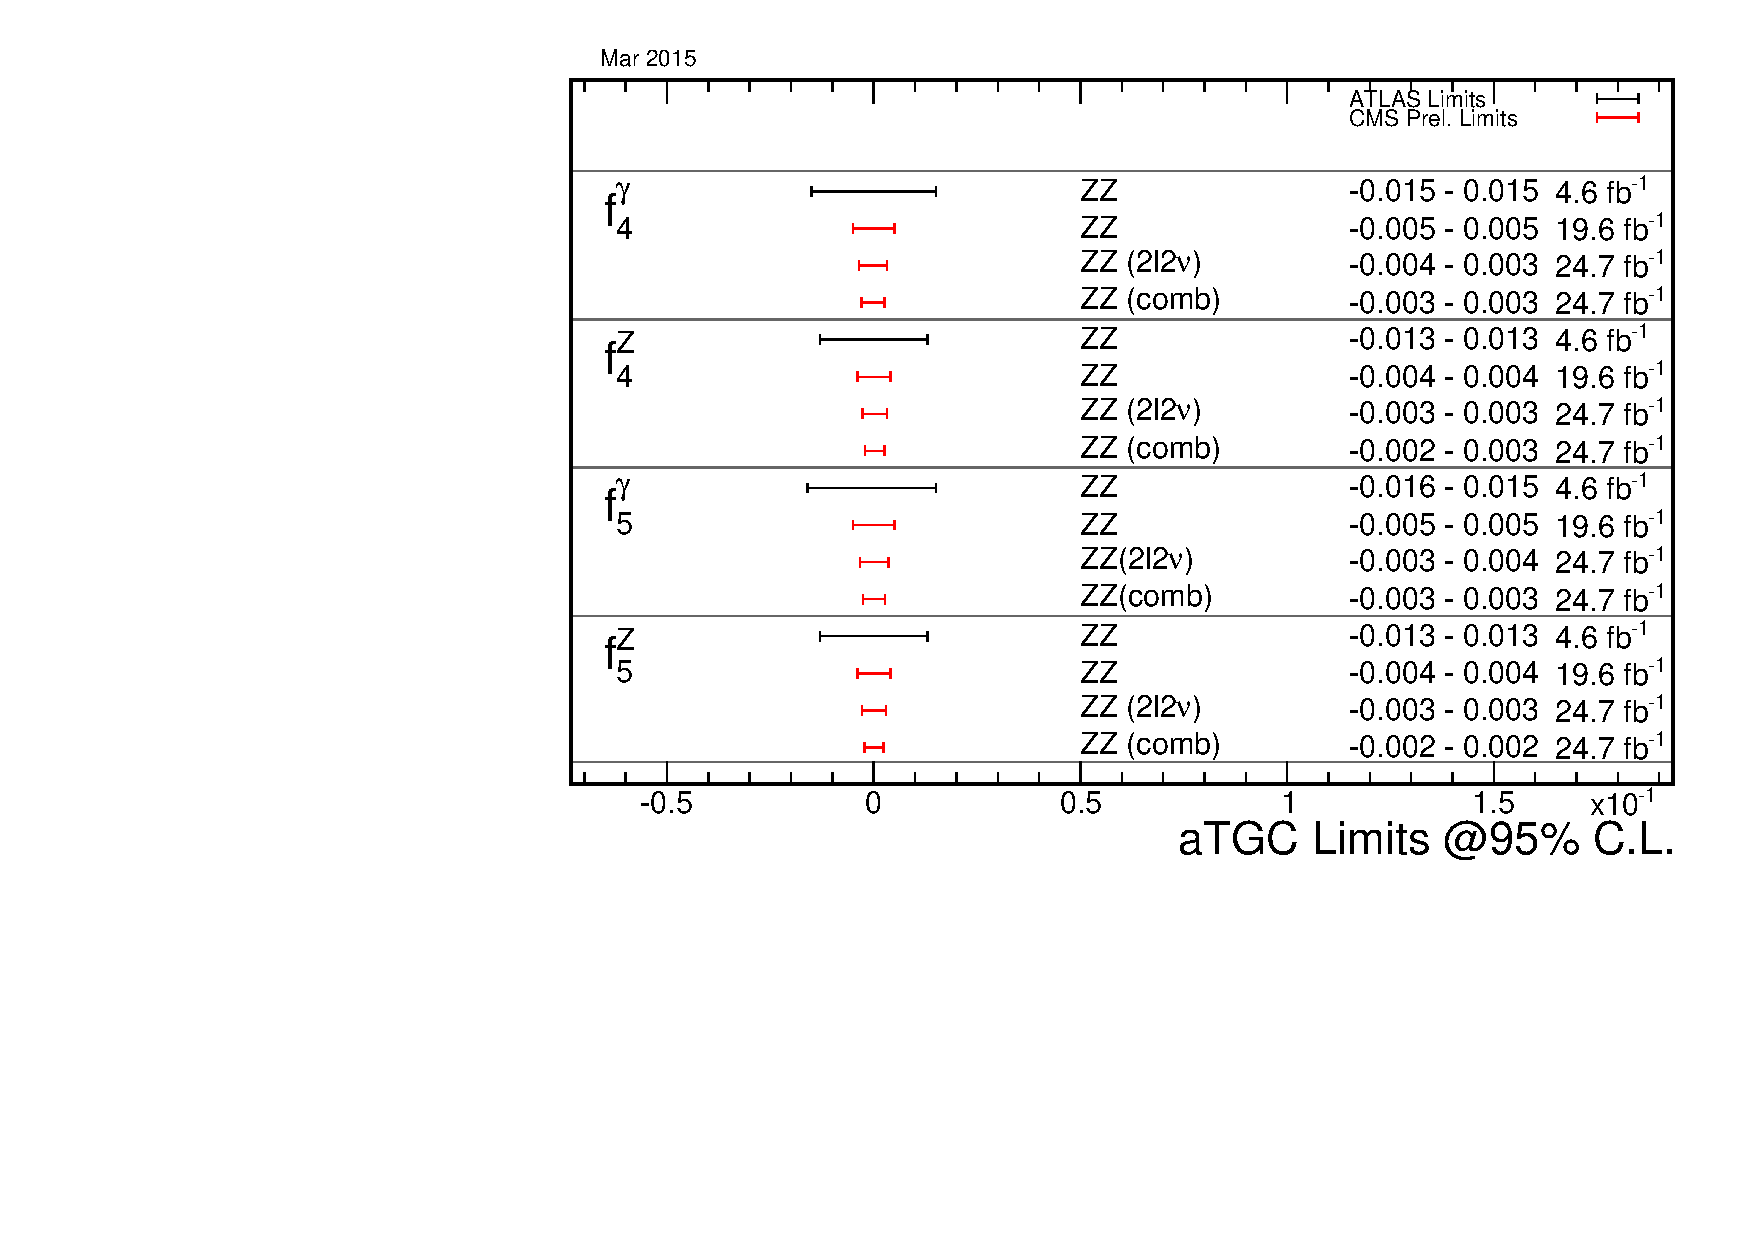
\includegraphics[width=0.6\textwidth]{figures/sss-inclboson-diboson-zzprod-aTGC_naTGCf.pdf}
  \caption{ Comparison of the limits on \ffourv{} and \ffivev{} from ATLAS and CMS in the $\ll\ll$ and $\ll\vv$
  channel at 7 and $8\TeV$~\cite{aTGCplots}.}
\label{fig:sss-inclboson-diboson-zzprod-aTGC_naTGCf}
\end{center}
\end{figure}







